\documentclass{article}

% Set page size and margins
% Replace `letterpaper' with `a4paper' for UK/EU standard size
\usepackage[a4paper,top=2cm,bottom=2cm,left=3cm,right=3cm,marginparwidth=2cm]{geometry}

% Language setting
% Replace `english' with e.g. `italian' to change the document language
\usepackage[english]{babel}

% Useful packages
\usepackage{amsmath}
\usepackage{mathspec}

\makeatletter % undo the wrong changes made by mathspec
\let\RequirePackage\original@RequirePackage
\let\usepackage\RequirePackage
\makeatother

\usepackage{tikz}
\usepackage{graphicx}
\usepackage{setspace}
\usepackage{multicol}
\usepackage[many]{tcolorbox}
\usepackage{algorithm}
\usepackage{algpseudocode}
\usepackage[colorlinks=true, allcolors=blue]{hyperref}

\usetikzlibrary{shapes,arrows,positioning,calc}

\newcounter{example}[section]
\newenvironment{example}[1][]{\refstepcounter{example}\par\medskip
   \noindent \textbf{Esempio~\theexample. #1} \rmfamily}{\medskip}

\newcounter{definition}[section]
\newenvironment{definition}[1][]{\refstepcounter{definition}\par\medskip
   \noindent \textbf{Definizione~\thedefinition. (#1)} \rmfamily}{\medskip}

\newcounter{fact}[section]
\newenvironment{fact}[1][]{\refstepcounter{fact}\par\medskip
   \noindent \textbf{Fact~\thefact. #1} \rmfamily}{\medskip}
   
\definecolor{main}{HTML}{5989cf}    % setting main color to be used
\definecolor{sub}{HTML}{cde4f9}     % setting sub color to be used

\tcbset{
    sharp corners,
    colback = white,
    before skip = 0.2cm,    % add extra space before the box
    after skip = 0.5cm      % add extra space after the box
}

\newtcolorbox{boxH}{
    colback = sub, 
    colframe = main, 
    boxrule = 0pt, 
    leftrule = 6pt % left rule weight
}

\title{Hash Functions}
\author{Federico Casu}

\begin{document}
\maketitle

\tikzset{
  block/.style = {draw, rectangle, text width=2.5cm, align=center, minimum height=1.5cm},
  arrow/.style = {thick,->,>=stealth},
  line/.style = {thick,-},
}

%%%%%%%%%%%%%%%%%%%%%%%%%%%%%%%%%%%%%%%%%%%%%%%%%%%%%%%%%%%%%%%%%%%%%%%%%%%%%%%%%%%%%%%%%%%%%%%%%%%%%%%%%%%%%%%%
\section{Introduzione}
Una funzione hash è una funzione matematica avente la seguente proprietà (informale):

\begin{boxH}
    Una funzione hash si definisce tale quando, per qualsiasi input, indipendentemente dalla sua lunghezza, la funzione restituisce un output di dimensione costante.
\end{boxH}

\par \noindent Formalizzare la proprietà che abbiamo appena citato è molto semplice:
\begin{equation*}
    \mathsf{H : \{0,1\}^* \rightarrow \{0,1\}^n}
\end{equation*}

\par In un contesto in cui la sicurezza è una priorità, le funzioni hash necessitano ulteriori proprietà. Facciamo un esempio:

\begin{example}
    Supponiamo di voler velocizzare il processo di firma digitale di un documento. Come ben sappiamo, la crittografia a chiave pubblica è 
    più lenta di 2 (talvolta 3) ordini di grandezza rispetto alla crittografia a chiave simmetrica. Per diminuire il costo della firma digitale 
    possiamo firmare il \textbf{digest} del documento, ovvero la firma digitale non viene apposta sull'intero documento ma su una stringa di bit, 
    quest'ultima di dimensione molto minori rispetto al documento, prodotta da una funzione hash.
\end{example}

\par \noindent Da questo esempio possiamo dedurre alcune proprietà legate alla sicurezza:

\begin{enumerate}
    \item La funzione hash deve essere \textit{one-way}, ovvero $\mathsf{H(x) = y}$ deve essere semplice da calcolare ma \underline{difficile} da 
    invertire ($\mathsf{H^{-1}(y) = x}$ deve essere computazionalmente infattibile).
    \item L'output della funzione, $\mathsf{H(x) = y}$, deve rappresentare univocamente l'input $\mathsf{x}$.
    \item La funzione hash non deve richiedere una chiave.
    \item Il digest prodotto dalla funzione hash deve essere sensibile ad ogni bit di input. In altre parole, si vorrebe che se due input 
    differiscono di un solo bit allora i rispettivi output (in media) differiscono in almeno la metà dei bits.
\end{enumerate}

\par \noindent Purtroppo, tra le proprietà sopra elencate, c'è ne una che matematicamente non è possibile ottenere: per definizione, 
una funzione hash è una funzione \textit{many-to-one}. Visto che il dominio della funzione ha una cardinalità maggiore del codominio, 
$\mathsf{\exists \text{ } x_{1} \neq x_2 \text{ tale che } H(x_1) = H(x_2)}$.

\par \noindent Al solito, siamo ingegneri, e ci accontentiamo di un po' meno rigore matematico a fronte di un approssimazione che nella pratica è 
verosimile.
%%%%%%%%%%%%%%%%%%%%%%%%%%%%%%%%%%%%%%%%%%%%%%%%%%%%%%%%%%%%%%%%%%%%%%%%%%%%%%%%%%%%%%%%%%%%%%%%%%%%%%%%%%%%%%%%

%%%%%%%%%%%%%%%%%%%%%%%%%%%%%%%%%%%%%%%%%%%%%%%%%%%%%%%%%%%%%%%%%%%%%%%%%%%%%%%%%%%%%%%%%%%%%%%%%%%%%%%%%%%%%%%%
\section{Funzioni Hash Sicure}
Prima di poter elencare le proprietà che rendono \textit{sicura} una funzione hash, dobbiamo definire il concetto di collisione.

\begin{definition}[Collisione]
    Si ha una \textit{collisione} quando esistono $\mathsf{x_1 \neq x_2}$ tali che $\mathsf{H(x_1) = H(x_2)}$.
\end{definition}

\noindent Perchè le collisioni sono nostre nemiche? Facciamo un esempio.

\begin{example}
    Supponiamo che Alice, per firmare un certo contratto di pagamento, abbia dovuto firmare il digest del documento. Bob, che è venuto a sapere
    ciò, vuole fare un dispetto ad Alice e scopre che il digest $\mathsf{y = H(x)}$ del contratto collide con un altro documento $\mathsf{x' \neq x}$, 
    avente lo stesso contenuto del documento originale ma accuratamente modificato nella somma di denaro ed in altre posizioni non visibili. 
    Bob potrebbe sostituire il contratto firmato da Alice con il contratto che lui, in mala fede, ha modificato: nessuno se ne accorgerebbe perchè
    \begin{equation*}
        \mathsf{H(x) = H(x') \rightarrow Sign(K_{priv}^{A}, H(x)) = Sign(K_{priv}^{A}, H(x'))}
    \end{equation*}
\end{example}

\begin{definition}[Pre-image resistance]
    Una funzione hash gode della proprietà di \textit{pre-image resistance} se, dato un digest $\mathsf{y}$ qualsiasi, è computazionalmente infattibile 
    calcolare $\mathsf{x}$ tale che $\mathsf{y = H(x)}$.
\end{definition}

\begin{definition}[Second pre-image resistance]
    Una funzione hash gode della proprietà di \textit{second pre-image resistance} se, dato $\mathsf{x_0}$ qualsiasi, è computazionalmente infattibile 
    trovare $\mathsf{x_1}$ tale che $\mathsf{H(x_0) = H(x_1)}$. Tale proprietà talvolta è detta \textit{weak collision resistance}.
\end{definition}

\begin{definition}[Collision resistance]
    Una funzione hash gode della proprietà di \textit{collision resistance} se è computazionalmente infattibile trovare una coppia $\mathsf{(x_0, x_1)}$, 
    $\mathsf{x_0 \neq x_1}$, tale che $\mathsf{H(x_0) = H(x_1)}$. Tale proprietà talvolta è detta \textit{strong collision resistance}.
\end{definition}

\begin{definition}[One-way hash function]
    Una funzione hash è detta \textit{one-way hash function} se gode della proprietà di \textit{pre-image resistance} e della proprietà 
    di \textit{second pre-image resitance}.
\end{definition} 

\begin{definition}[Cryptographically Secure hash function]
    Una funzione hash è detta \textit{cryptographically secure hash function} se gode delle proprietà di \textit{second pre-image resitance} 
    e \textit{collision resistance}.
\end{definition}

\begin{fact}[Collision resistance $\rightarrow$ 2nd pre-image resistance]
    Se una funzione hash gode della proprietà di \textit{collision resistance} allora gode anche della proprietà di \textit{second pre-image resistance} 
    (strong collision resistance implica weak collision resistance, non è vero il contrario).
\end{fact}

\begin{fact}
    Se una funzione hash gode della proprietà di \textit{collision resistance} non è detto che goda anche della proprietà di 
    \textit{pre-image resistance} (strong collision resistance \underline{non} implica pre-image resistance).
\end{fact}
%%%%%%%%%%%%%%%%%%%%%%%%%%%%%%%%%%%%%%%%%%%%%%%%%%%%%%%%%%%%%%%%%%%%%%%%%%%%%%%%%%%%%%%%%%%%%%%%%%%%%%%%%%%%%%%%

%%%%%%%%%%%%%%%%%%%%%%%%%%%%%%%%%%%%%%%%%%%%%%%%%%%%%%%%%%%%%%%%%%%%%%%%%%%%%%%%%%%%%%%%%%%%%%%%%%%%%%%%%%%%%%%%
\section{Attacchi di tipo \textit{black box}}
Sia nella crittografia a chiave simmetrica, sia nella crittografia a chiave pubblica, abbiamo potuto notare il 
fatto che è sempre possibile eseguire un attacco a \textit{forza bruta}. Questa tipologia di attacchi consistono 
nel trattare l' \textit{encryption scheme} come una scatola nera che prende in ingresso un messaggio in chiaro e 
restituisce il messaggio cifrato corrispondente diverso a seconda della chiave di cifratura utilizzata. Le funzioni 
hash possono essere attaccate: l'obiettivo dell'attacante è ottenere una collisione.

\par Supponiamo di voler invertire una funzione hash, ovvero vorremo ottenere l'input $\mathsf{x}$ che ha 
prodotto il digest $\mathsf{y}$. L'attacco è il seguente:

\begin{algorithm}
    \caption{Guessing Attack}
    \label{alg:black_box_attack}
    \begin{algorithmic}
        \Repeat
            \State $\mathsf{x \gets random()}$
        \Until{$\mathsf{H(x) == y}$}
    \end{algorithmic}
\end{algorithm}

\par Qual'è la complessità dell'algoritmo? Dipende dalla dimensione dell'output: visto che il codominio ha 
cardinalità $\mathsf{Card \left( \{0,1\}^n \right) = 2^n}$, al più la funzione hash è in grado di generare 
$\mathsf{2^n}$ output distinti. Ciò significa che per trovare $\mathsf{x}$ tale che $\mathsf{y = H(x)}$ 
è necessario, in media, eseguire $\mathsf{O(2^n)}$ iterazioni.

\par \noindent Si presti attenzione al fatto che i black box attacks rappresentano solamente un limite superiore. 
In altre parole, i black box attacks ci dicono che peggio di così non possiamo fare. Purtroppo non possiamo assumere 
che la complessità di un algoritmo in grado di rompere una funzione hash sia $\mathsf{O(2^n)}$ perchè non possiamo 
affermare con certezza che non esistano attacchi più efficienti. \newline

\par \noindent Possiamo suddividere la classe degli attacchi alle funzioni hash in due sottoclassi:

\begin{enumerate}
    \item \textbf{Existential forgery}: l'attacante non ha controllo sull'input $\mathsf{x}$.
    \item \textbf{Selective forgery}: l'attacante ha completo (o parziale) controllo sull'input $\mathsf{x}$.
\end{enumerate}

\subsection{Birthday attack}
Le funzioni hash, indipendentemente dal loro design, possono essere soggette ad una tipologia di attacco la 
cui complessità è $\mathsf{O(2^{n/2})}$!

\par \noindent Prendiamo in esame i seguenti semplici problemi di probabilità, apparantemente scollegati dal 
mondo delle funzioni hash, ma che in seguito si riveleranno fondamentali.

\begin{example}
    Si consideri un insieme di $\mathsf{t = 23}$ persone. Qual'è la probabilità che almeno una persona sia 
    nata il 25 Dicembre? \newline
    \textit{Soluzione}: l'evento $\mathsf{E = }$ "almeno una persona del gruppo è nata il 25 Dicembre" è 
    dato dall'unione degli eventi "persona $\mathsf{j}$ nata il 25 Dicembre", $\mathsf{j = 1, ..., 23}$. 
    Ciascun evento è indipendentemente e disgiunto dagli altri. Segue che la probabilità può essere calcolata come:
    \begin{equation*}
        \mathsf{P(E) = \sum_{j = 1}{23} \frac{1}{365} = \frac{23}{365} = 0.063}
    \end{equation*}
\end{example}

\begin{example}[(Birthday Paradox)]
    Si consideri un insieme di $\mathsf{t = 23}$ persone. Qual'è la probabilità che almeno due 
    persone siano nate nello stesso giorno? \newline
    \textit{Soluzione}: possiamo calcolare la probabilità $\mathsf{P(E)}$ come $\mathsf{P(E) = 1 - P(Q)}$, 
    dove $\mathsf{Q}$ è l'evento "nessun individuo è nato lo stesso giorno di un altro individuo".
    \begin{equation*}
        \mathsf{P(e) = 1 - \left(1 - \frac{1}{365} \right) \cdot \left(1 - \frac{2}{365} \right) \cdot \dots \cdot \left(1 - \frac{22}{365} \right) = 0.507}
    \end{equation*}
\end{example}

\par \noindent Notiamo che la probabilità dell'evento $\mathsf{Q = \exists}$ $\mathsf{2}$ $\mathsf{persone}$ $\mathsf{nate}$ $\mathsf{lo \text{ } stesso}$ 
$\mathsf{giorno}$ è, circa, di un ordine di grandezza maggiore rispetto alla probabilità del primo 
problema. Questi due semplici problemi ci permettono di capire che esiste una seconda tipologia di 
attacco la cui complessità è nell'ordine di $\mathsf{O(2^{n/2})}$.

\begin{fact}
    Il problema $\mathsf{Birthday \text{ } Paradox}$ è equivalente al seguente problema: qual'è 
    la probabilità di trovare una coppia $\mathsf{\langle x_0, x_1\rangle}$, $\mathsf{x_0, \neq x_1}$, $\mathsf{H(x_0) = H(x_1)}$.
\end{fact}  

\noindent Di fatto, possiamo paragonare il numero di persone presenti nella sala in cui si svolge la 
narrazione del $\mathsf{Birthday \text{ } Paradox}$ al numero di tentativi compiuti per trovare una 
collisione a partire da una coppia di input qualsiasi. Il passo successivo è il calcolo del numero di 
tentativi necessari per forgiare una collisione:

\begin{align*}
    \mathsf{P(Q)} &= \mathsf{\left(1 - \frac{1}{2^n} \right) \cdot \left(1 - \frac{2}{2^n} \right) \cdot \dots \cdot \left(1 - \frac{t-1}{2^n} \right)} = \\
    &= \mathsf{\prod_{j=1}^{t-1} \left(1 - \frac{j}{2^n} \right)} \\
\end{align*}

Ora applichiamo una approssimazione: $\mathsf{1-x \approx e^{-x} \text{ se } x << 1}$. Segue:
\begin{align*}
    \mathsf{P(Q)} &= \mathsf{\prod_{j=1}^{t-1} \left(1 - \frac{j}{2^n} \right)} \approx \\
    &\approx \mathsf{\prod_{j=1}^{t-1} e^{- \frac{j}{2^n}}} = \\ 
    &= \mathsf{ e^{- \left( \frac{1}{2^n} + \frac{2}{2^n} + \dots + \frac{t-1}{2^n} \right) } } = \\
    &= \mathsf{ e^{- \frac{1 + 2 + \dots + t-1}{2^n} }} = \\
    &= \mathsf{ e^{- \frac{t(t-1)}{2 \cdot 2^n} }} \approx \\ 
    &\approx \mathsf{ e^{- \frac{t^2}{2 \cdot 2^n} }} 
\end{align*}

\noindent Adesso vogliamo dare un valore all'incognita $\mathsf{t}$: quanti tentativi è necessario compiere 
per ottenere una collisione con una certa probabilità $\mathsf{\lambda}$?

\begin{align*}
    \mathsf{P(Q)} &\approx \mathsf{ e^{- \frac{t^2}{2 \cdot 2^n} }}                   \\ 
    \mathsf{P(E)} &= \mathsf{1 - P(Q)} = \mathsf{ 1 - e^{- \frac{t^2}{2 \cdot 2^n} }} \\
    & \text{supponiamo } \mathsf{P(E) = \lambda}                                      \\
    &\mathsf{ 1 - e^{- \frac{t^2}{2 \cdot 2^n} }} = \mathsf{\lambda}                  \\
    &\mathsf{e^{- \frac{t^2}{2 \cdot 2^n} }} = \mathsf{1 - \lambda}                   \\
    &\mathsf{- \frac{t^2}{2 \cdot 2^n} } = \mathsf{log(1 - \lambda)}                  \\
    &\mathsf{\frac{t^2}{2 \cdot 2^n} } = \mathsf{log(\frac{1}{1 - \lambda})}          \\
    &\mathsf{t^2} = \mathsf{2^{n+1} log(\frac{1}{1 - \lambda})}                       \\
    &\mathsf{t} = \mathsf{\sqrt{ 2^{n+1} log(\frac{1}{1 - \lambda}) }}                \\
    &\mathsf{t} = \mathsf{2^{\frac{n+1}{2}} \sqrt{log(\frac{1}{1 - \lambda})}}
\end{align*}

\noindent Cosa possiamo notare? Il parametro $\mathsf{\lambda}$ è pressochè ininfluente: l'ordine del numero di 
operazioni è dato da $\mathsf{2^{\frac{n+1}{2}}}$. Il numero di messaggi che dobbiamo hashare per trovare una 
collisione è dell'ordine della radice quadrata della cardinalità del codominio, ovvero $\mathsf{O(2^{n/2})}$.
%%%%%%%%%%%%%%%%%%%%%%%%%%%%%%%%%%%%%%%%%%%%%%%%%%%%%%%%%%%%%%%%%%%%%%%%%%%%%%%%%%%%%%%%%%%%%%%%%%%%%%%%%%%%%%%%

%%%%%%%%%%%%%%%%%%%%%%%%%%%%%%%%%%%%%%%%%%%%%%%%%%%%%%%%%%%%%%%%%%%%%%%%%%%%%%%%%%%%%%%%%%%%%%%%%%%%%%%%%%%%%%%%
\section{Come costruire una funzione hash}
\par \noindent Finora abbiamo discusso i requisiti delle funzioni di hash. Ora introduciamo come costruirle effettivamente. 
Esistono due possibili approcci:

\begin{enumerate}
    \item \textbf{Funzioni hash dedicate}. Questi sono algoritmi appositamente progettati per funzionare come funzioni hash.
    \item \textbf{Funzioni hash basate su cifrari a blocchi}. Si possono utilizzare cifrari a blocchi (esempio: $\mathsf{AES}$) per costruire funzioni hash.
\end{enumerate}

\noindent Come abbiamo visto nelle sezioni precedenti, le funzioni hash possono elaborare un messaggio di lunghezza 
arbitraria e produrre un output di lunghezza fissa. Nella pratica, ciò è ottenuto suddividendo l'input in una serie 
di blocchi di dimensioni uguali. Questi blocchi vengono elaborati sequenzialmente dalla funzione hash: ciascun blocco 
diventa l'input di una funzione, detta $\mathsf{funzione \text{ } di \text{ } compressione}$, insiem al digest ottenuto 
dal blocco precedente. Questo design è noto come costruzione di $\mathsf{Merkle\text{-}Damgard}$. L' hash del messaggio 
in ingresso è quindi definito come l'output dell'ultima iterazione della funzione di compressione.

\begin{figure}
    \centering
    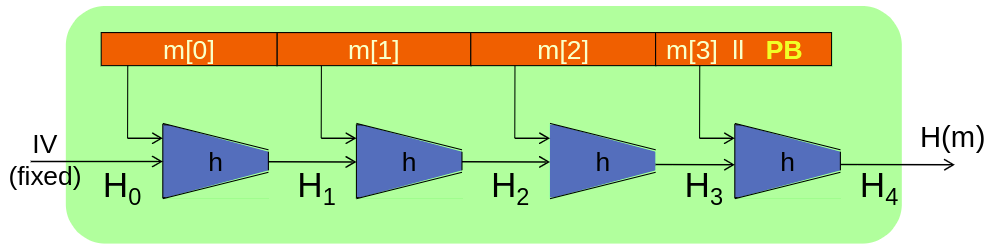
\includegraphics[width=0.65\linewidth]{figures/merkle-damgard.png}
    \caption{\label{fig:merkle_damgard}Merkle-Damgard design.}
\end{figure}
%%%%%%%%%%%%%%%%%%%%%%%%%%%%%%%%%%%%%%%%%%%%%%%%%%%%%%%%%%%%%%%%%%%%%%%%%%%%%%%%%%%%%%%%%%%%%%%%%%%%%%%%%%%%%%%%



\end{document}
